\documentclass[
11pt, % The default document font size, options: 10pt, 11pt, 12pt
%codirector, % Uncomment to add a codirector to the title page
]{charter} 


% El títulos de la memoria, se usa en la carátula y se puede usar el cualquier lugar del documento con el comando \ttitle
\titulo{Sistema IoT para el Monitoreo de Niveles de Ruido en Entornos Cerrados o Pequeñas Áreas Urbanas} 

% Nombre del posgrado, se usa en la carátula y se puede usar el cualquier lugar del documento con el comando \degreename
\posgrado{Carrera de Especialización en Internet de las Cosas} 
%\posgrado{Carrera de Especialización en Internet de las Cosas} 
%\posgrado{Carrera de Especialización en Inteligencia Artificial}
%\posgrado{Maestría en Sistemas Embebidos} 
%\posgrado{Maestría en Internet de las cosas}

% Tu nombre, se puede usar el cualquier lugar del documento con el comando \authorname
% IMPORTANTE: no omitir titulaciones ni tildación en los nombres, también se recomienda escribir los nombres completos (tal cual los tienen en su documento)
\autor{Ing. José Pedro Rivero Peña}

% El nombre del director y co-director, se puede usar el cualquier lugar del documento con el comando \supname y \cosupname y \pertesupname y \pertecosupname
\director{Título y Nombre del director}
\pertenenciaDirector{pertenencia} 
\codirector{} % para que aparezca en la portada se debe descomentar la opción codirector en los parámetros de documentclass
\pertenenciaCoDirector{FIUBA}

% Nombre del cliente, quien va a aprobar los resultados del proyecto, se puede usar con el comando \clientename y \empclientename
\cliente{Nombre del cliente}
\empresaCliente{-}
 
\fechaINICIO{04 de marzo de 2025}		%Fecha de inicio de la cursada de GdP \fechaInicioName
\fechaFINALPlan{22 de abril de 2025} 	%Fecha de final de cursada de GdP
\fechaFINALTrabajo{15 de octubre de 2025}	%Fecha de defensa pública del trabajo final


\begin{document}

\maketitle
\thispagestyle{empty}
\pagebreak


\thispagestyle{empty}
{\setlength{\parskip}{0pt}
\tableofcontents{}
}
\pagebreak


\section*{Registros de cambios}
\label{sec:registro}


\begin{table}[ht]
\label{tab:registro}
\centering
\begin{tabularx}{\linewidth}{@{}|c|X|c|@{}}
\hline
\rowcolor[HTML]{C0C0C0} 
Revisión & \multicolumn{1}{c|}{\cellcolor[HTML]{C0C0C0}Detalles de los cambios realizados} & Fecha      \\ \hline
0      & Creación del documento                                 &\fechaInicioName \\ \hline
1      & Se completa hasta el punto 5 inclusive                & {20} de {mayo} de 2025 \\ \hline
2      & Se completa hasta el punto 9 inclusive                & {28} de {mayo} de 2025 \\ \hline
3      & Se completa hasta el punto 12 inclusive                & {06} de {abril} de 2025 \\ \hline
%4      & Se completa el plan	                                 & {día} de {mes} de 202X \\ \hline

% Si hay más correcciones pasada la versión 4 también se deben especificar acá

\end{tabularx}
\end{table}

\pagebreak



\section*{Acta de constitución del proyecto}
\label{sec:acta}

\begin{flushright}
Buenos Aires, \fechaInicioName
\end{flushright}

\vspace{2cm}

Por medio de la presente se acuerda con el \authorname\hspace{1px} que su Trabajo 
Final de la \degreename\hspace{1px} se titulará ``\ttitle'' y consistirá en la implementación de un prototipo de un sistema 
IoT para el monitoreo de niveles de ruido en entornos cerrados o pequeñas áreas urbanas. El trabajo tendrá un presupuesto 
preliminar estimado de {600} horas y un costo estimado de 240.000 ARS, con fecha de inicio el \fechaInicioName\hspace{1px} y fecha de presentación pública el \fechaFinalName.

Se adjunta a esta acta la planificación inicial.

\vfill

% Esta parte se construye sola con la información que hayan cargado en el preámbulo del documento y no debe modificarla
\begin{table}[ht]
\centering
\begin{tabular}{ccc}
\begin{tabular}[c]{@{}c@{}}Dr. Ing. Ariel Lutenberg \\ Director posgrado FIUBA\end{tabular} & \hspace{2cm} & \begin{tabular}[c]{@{}c@{}}\clientename \\ \empclientename \end{tabular} \vspace{2.5cm} \\ 
\multicolumn{3}{c}{\begin{tabular}[c]{@{}c@{}} \supname \\ Director del Trabajo Final\end{tabular}} \vspace{2.5cm} \\
\end{tabular}
\end{table}




\section{1. Descripción técnica-conceptual del proyecto a realizar}
\label{sec:descripcion}

El monitoreo de los niveles acústicos en entornos cerrados y pequeños espacios urbanos es un problema que no se puede dejar de
 lado en la sociedad actual. La exposición constante a altos niveles de ruido puede generar estrés, fatiga auditiva y afectar 
 la concentración y productividad en oficinas, hospitales, aulas y parques. A pesar de la existencia de sistemas de medición 
 de ruidos, estos suelen ser costosos, estacionarios o requieren intervención manual para la toma y análisis de datos. En este 
 contexto, surge la necesidad de desarrollar soluciones tecnológicas accesibles, autónomas y escalables para la medición en 
 tiempo real de los niveles de ruido ambiental.

 Este proyecto propone el desarrollo de un sistema IoT capaz de monitorear el nivel de ruido en tiempo real, mediante sensores 
 que recopilan la información y la transmiten a una plataforma en la nube. De este modo, los usuarios pueden acceder a los 
 datos y gestionar alertas asociadas a parámetros definidos. A diferencia de soluciones tradicionales, esta propuesta se 
 enfoca en la modularidad y accesibilidad, permitiendo su implementación en diversos entornos sin necesidad de grandes 
 inversiones en infraestructura.
 La solución contempla el uso de sensores calibrados, microcontroladores con conectividad inalámbrica y un sistema de 
 almacenamiento y visualización de datos basado en la nube, lo que facilita el acceso a la información desde cualquier 
 dispositivo con conexión a internet. La propuesta se diferencia de las existentes al integrar alertas configurables, 
 escalabilidad para expansión del sistema y la posibilidad de incorporar algoritmos de inteligencia artificial en futuras 
 fases para la identificación de patrones de ruido y predicción de niveles sonoros.

 El sistema propuesto consta de varios módulos funcionales. En primer lugar, los nodos sensores distribuidos miden el nivel 
 de ruido en diferentes ubicaciones y procesan localmente los datos antes de enviarlos a través de una red de comunicación 
 Wi-Fi en entornos con infraestructura disponible y LoRa en espacios abiertos sin acceso a redes tradicionales. Los datos 
 recopilados son almacenados en la nube y pueden visualizarse en una interfaz web, donde los usuarios pueden consultar 
 registros históricos, recibir alertas en tiempo real y tomar decisiones en función de la información proporcionada por el 
 sistema. Además, la optimización energética es un aspecto clave del diseño, por lo que los dispositivos funcionarán con 
 baterías de larga duración y, en casos específicos, podrán incorporar alimentación solar para garantizar una operación continua.

 Uno de los principales desafíos del proyecto es garantizar la precisión y confiabilidad de las mediciones en distintos 
 entornos, para lo que se ha considerado la incorporación de un segundo tipo de sensor para controlar factores ambientales 
 como temperatura y humedad, que pueden influir en la propagación del sonido. Asimismo, se busca desarrollar un sistema que 
 pueda expandirse fácilmente, permitiendo la incorporación de nuevos nodos de medición sin afectar el rendimiento general de 
 la plataforma. La seguridad en la transmisión y almacenamiento de los datos también es un aspecto crítico, por lo que se 
 emplearán protocolos de comunicación seguros como MQTT con cifrado.

 Este emprendimiento personal busca proporcionar una herramienta útil para el monitoreo de ruido en espacios donde el control 
 acústico es un factor clave para la calidad de vida. La facilidad de implementación y la flexibilidad del sistema permiten 
 su aplicación en múltiples sectores, desde instituciones educativas y hospitales hasta gobiernos municipales interesados en 
 gestionar la contaminación acústica en espacios públicos. Con una infraestructura abierta y escalable, este sistema puede 
 evolucionar para integrar nuevas funcionalidades.

 A continuación, se presenta el diagrama del sistema, en el que se ilustra la interacción entre sus diferentes componentes y el 
 flujo de datos desde la captación hasta la visualización de los datos.


\begin{figure}[htpb]
	\centering 
	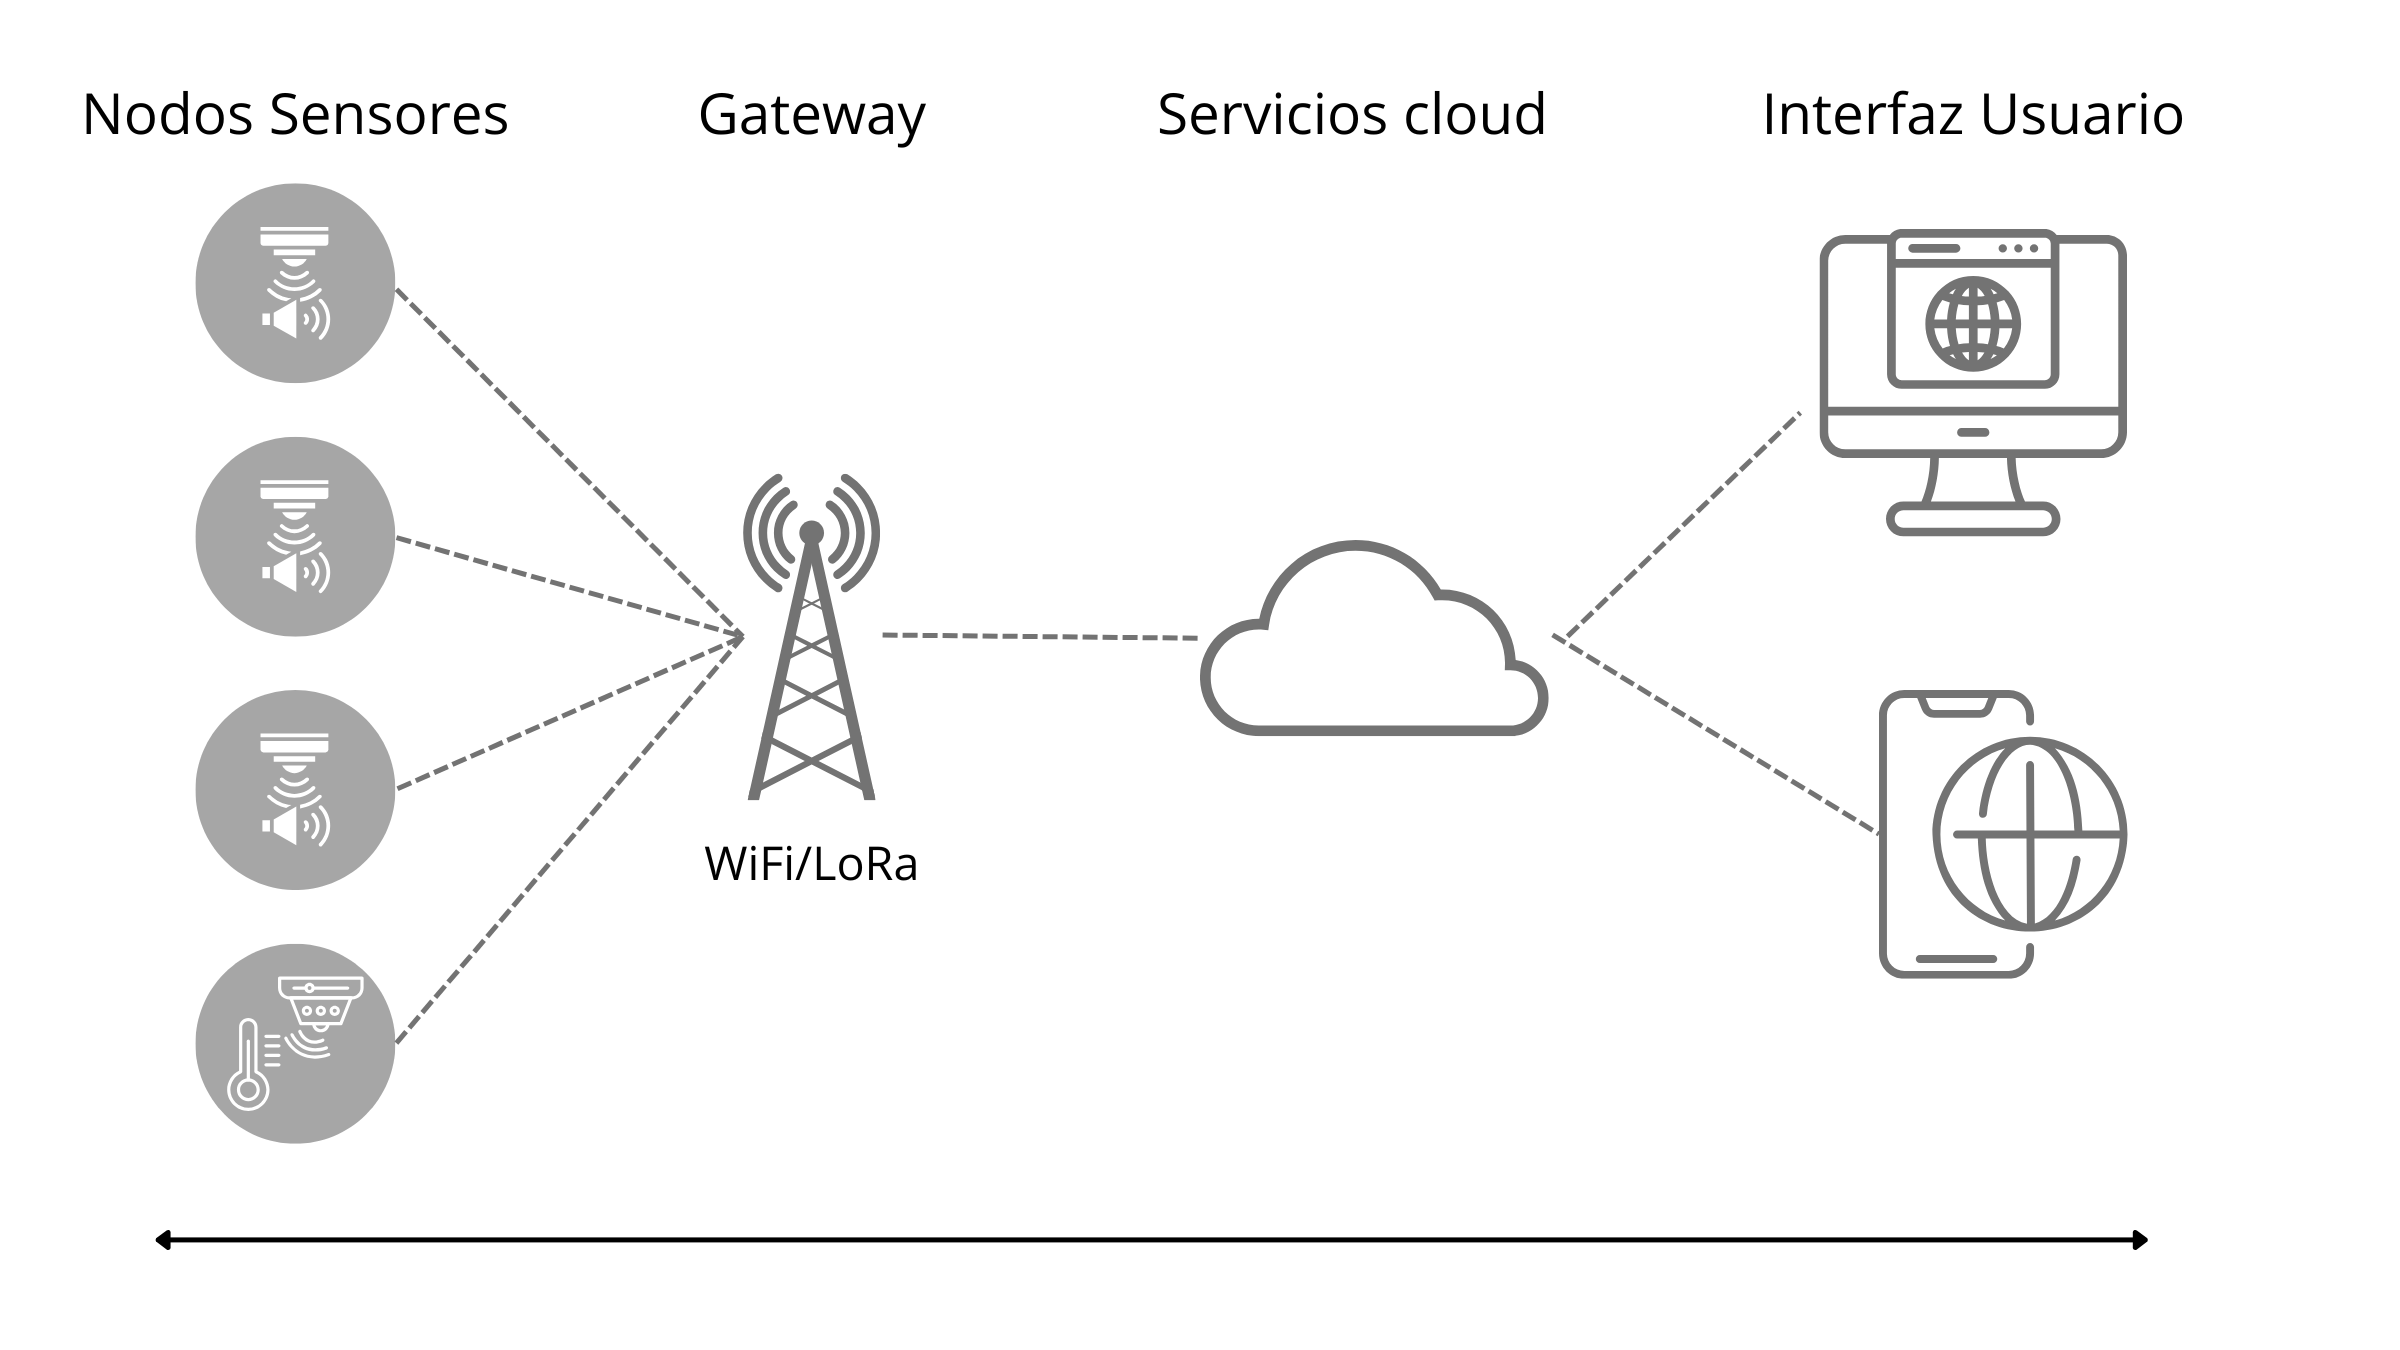
\includegraphics[width=.65\textwidth]{./Figuras/diagramaSist.png}
	\caption{Diagrama del sistema.}
	\label{fig:diagBloques}
	\end{figure}
	
	\vspace{25px}

\section{2. Identificación y análisis de los interesados}
\label{sec:interesados}



\begin{table}[ht]
%\caption{Identificación de los interesados}
%\label{tab:interesados}
\begin{tabularx}{\linewidth}{@{}|l|X|X|l|@{}}
\hline
\rowcolor[HTML]{C0C0C0} 
Rol           & Nombre y Apellido & Organización 	& Puesto 	\\ \hline
Auspiciante   &       -           &       -       	&      -  	\\ \hline
Cliente       & \clientename      &\empclientename	&       - 	\\ \hline
Impulsor      &      -             &     -         	&     -   	\\ \hline
Responsable   & \authorname       & FIUBA        	& Alumno 	\\ \hline
Colaboradores &      -             &        -      	&     -   	\\ \hline
Orientador    & \supname	      & \pertesupname 	& Director del Trabajo Final \\ \hline
Equipo        & Por definir \newline 
				Por definir         &      Por definir         	&   Por definir      	\\ \hline
Opositores    &     -              &       -       	&     -   	\\ \hline
Usuario final &  Gobiernos, empresas y civiles                &         -     	&        -	\\ \hline
\end{tabularx}
\end{table}



\section{3. Propósito del proyecto}
\label{sec:proposito}
 
Desarrollar un sistema IoT eficiente, escalable y de bajo costo para la medición y monitoreo en tiempo real de los niveles de 
ruido en entornos cerrados y pequeñas áreas urbanas que permita recopilar, procesar y visualizar datos acústicos de manera 
accesible. Capz de proporcionar a los usuarios información precisa sobre la contaminación sonora en distintos espacios. 
\section{4. Alcance del proyecto}
\label{sec:alcance}

La propuesta está orientada a ofrecer un sistema modular, escalable y de bajo consumo energético, con una infraestructura 
adaptable a distintos escenarios de uso.

\clearpage
El proyecto incluye:
\begin{itemize}
    \item \textbf{Diseño e implementación de un sistema IoT para monitoreo de ruido}, compuesto por nodos sensores, un módulo de comunicación y una plataforma en la nube.
    \begin{itemize}
        \item Desarrollo de un prototipo funcional con tres nodos sensores distribuidos en un entorno de prueba.
        \item Selección, calibración y configuración de sensores de ruido con un rango de medición entre 30 y 120 dB, 
        que garantice una precisión aceptable para el análisis acústico.
        \item Integración con microcontrolador esp32 que permita el procesamiento de datos en la transmisión de información.
        \item Implementación de un módulo de conectividad inalámbrica utilizando tecnologías Wi-Fi para entornos cerrados y LoRa para áreas urbanas con baja cobertura de red.
    \end{itemize}
    
    \item \textbf{Desarrollo de una plataforma en la nube para almacenamiento y visualización de datos.}
    \begin{itemize}
        \item Configuración de una base de datos para el almacenamiento de registros históricos y análisis posterior.
        \item Implementación de un dashboard web accesible para la consulta de datos en tiempo real, que permita la visualización de mediciones y tendencias históricas.
        \item Incorporación de un sistema de alertas configurables para notificar a los usuarios cuando los niveles de ruido superen los umbrales predefinidos.
    \end{itemize}
    
    \item \textbf{Optimización energética del sistema}, asegurando bajo consumo y autonomía en los nodos sensores.
    \begin{itemize}
        \item Implementación de estrategias de bajo consumo en los microcontroladores, utilizando modos de suspensión y transmisión periódica.
        \item Evaluación del uso de baterías recargables con posibilidad de integración de paneles solares en escenarios de monitoreo prolongado.
    \end{itemize}
    
\end{itemize}

El presente proyecto no incluye:
\begin{itemize}
    \item Reducción o mitigación del ruido ambiental, ya que su enfoque se limita a la medición y análisis de los niveles de ruido.
    \item Integración con modelos de inteligencia artificial o análisis predictivo en esta fase inicial, aunque el sistema está diseñado para futuras ampliaciones en este sentido.
    \item Desarrollo de una aplicación móvil nativa; el acceso a los datos y la visualización del sistema se realizarán únicamente a través de una interfaz web.
    \item Implementación en escenarios reales fuera del alcance de pruebas controladas, limitándose en esta etapa a un entorno de prueba definido para la validación del prototipo.
\end{itemize}

\section{5. Supuestos del proyecto}
\label{sec:supuestos}

Para el desarrollo del presente proyecto se supone que:

\begin{itemize}
    \item No se considerarán regulaciones específicas sobre privacidad o normativas de manejo de datos, dado que el sistema solo recopilará información de niveles de ruido sin asociarlos a datos personales o identificables.
    \item Se asumirá que las condiciones de infraestructura en los entornos de prueba son representativas de espacios urbanos y cerrados típicos, sin interferencias extremas que afecten la captura y transmisión de datos.
    \item Se dispondrá de una red eléctrica estable en las áreas de prueba, que permita el funcionamiento de los sensores y la transmisión de datos sin interrupciones críticas.
    \item No se considerarán eventos extremos como fallos masivos de red, cortes prolongados de energía o interferencias radioeléctricas severas que puedan comprometer el funcionamiento del sistema.
    \item Se asumirá que las condiciones ambientales dentro de los entornos de prueba serán normales, sin presencia de factores climáticos extremos que puedan afectar la medición del sonido o el funcionamiento de los dispositivos.
    \item Se trabajará con un conjunto limitado de nodos sensores, sin escalabilidad masiva en esta fase del proyecto.
    \item No se contemplará la implementación de sistemas de redundancia avanzada para la transmisión y almacenamiento de datos, ya que el proyecto busca validar la funcionalidad básica del sistema en su fase inicial.
\end{itemize}


\section{6. Requerimientos}
\label{sec:requerimientos}

\section{Requerimientos del Proyecto}

A continuación, se enumeran los requerimientos del sistema propuesto.

\begin{enumerate}
    \item \textbf{Requerimientos funcionales (prioridad alta):}
    \begin{enumerate}
        \item El sistema debe medir niveles de ruido ambiental en tiempo real con una frecuencia configurable (mínimo una medición cada 5 minutos).
        \item Los sensores deben registrar valores en dB con un rango de 30–120 dB y precisión máxima de ±2 dB.
        \item El microcontrolador debe procesar localmente los datos y transmitirlos a la nube usando Wi-Fi o LoRaWan, según el entorno.
        \item El sistema debe generar una alerta automática cuando el nivel de ruido supere un umbral configurable.
        \item El sistema debe permitir almacenar los datos de manera estructurada y persistente en una base de datos alojada en un servidor remoto.
        \item El usuario debe poder acceder a los datos mediante un dashboard web desde cualquier navegador moderno.
        \item El sistema debe estar probado en un entorno controlado como prueba de concepto, con documentación del despliegue y resultados.
    \end{enumerate}

    \item \textbf{Requerimientos de interfaz (prioridad alta):}
    \begin{enumerate}
        \item El usuario debe poder acceder a un dashboard web desde navegadores modernos sin necesidad de instalar software adicional.
        \item La interfaz debe mostrar los niveles de ruido actuales, valores históricos y tendencias de forma visual y comprensible (por ejemplo, gráficos de líneas, colores de alerta, etc.).
        \item El usuario debe poder configurar el umbral de alertas desde la misma interfaz.
    \end{enumerate}

    \item \textbf{Requerimientos de hardware (prioridad alta):}
    \begin{enumerate}
        \item Cada nodo debe operar al menos 5 días seguidos con batería sin recarga (con opción de carga solar).
        \item Los sensores deben ser fácilmente reemplazables o reubicables.
        \item El sistema debe funcionar en ambientes interiores y exteriores moderadamente protegidos.
    \end{enumerate}

    \item \textbf{Requerimientos de backend y almacenamiento (prioridad alta):}
    \begin{enumerate}
        \item La base de datos utilizada deberá permitir el almacenamiento estructurado de registros históricos con acceso rápido (PostgreSQL o SQLite en entorno cloud).
    \end{enumerate}

    \item \textbf{Requerimientos de interoperabilidad (prioridad baja, opcional):}
    \begin{enumerate}
        \item El sistema podrá exportar los datos en formato CSV o JSON para análisis externo (requerimiento opcional).
    \end{enumerate}

    \item \textbf{Requerimientos de seguridad (prioridad media):}
    \begin{enumerate}
        \item El acceso al dashboard debe estar protegido mediante credenciales de usuario.
        \item El backend debe implementar un sistema básico de autenticación, como JWT o similar, para proteger las rutas de acceso a datos.
        \item Las comunicaciones entre el nodo y el servidor deben utilizar protocolos seguros, salvo en casos justificados por limitaciones técnicas.
    \end{enumerate}

    \item \textbf{Requerimientos normativos (prioridad alta):}
    \begin{enumerate}
        \item El sistema debe contemplar los valores límite de exposición al ruido establecidos por la Ley N.º 1540 de la Ciudad Autónoma de Buenos Aires.
        \item Las alertas deberán configurarse con base en dichos umbrales: 55 dB para interiores diurnos, 45 dB para nocturnos, 70 dB en espacios públicos al aire libre.
    \end{enumerate}
\end{enumerate}

\section{7. Historias de usuarios (\textit{Product backlog})}
\label{sec:backlog}

\section{Historias de Usuario}

\begin{enumerate}
    \item \textbf{Como administrador del sistema quiero visualizar en un panel web los niveles actuales de ruido en tiempo real para monitorear el estado acústico del entorno.}

    \textit{Story points}: 8 (complejidad: 3, dificultad: 2, incertidumbre: 2)
    \clearpage
    \textbf{Criterios de aceptación}:
    \begin{itemize}
        \item El dashboard debe mostrar los valores actuales de dB por nodo sensor.
        \item La información debe actualizarse automáticamente cada 5 minutos o menos.
        \item El diseño debe ser claro, responsivo y accesible desde cualquier navegador moderno.
    \end{itemize}

    \item \textbf{Como usuario del sistema quiero recibir una alerta cuando el nivel de ruido supere un umbral definido para poder tomar acciones correctivas.}

    \textit{Story points}: 8 (complejidad: 2, dificultad: 2, incertidumbre: 2)

    \textbf{Criterios de aceptación}:
    \begin{itemize}
        \item El usuario podrá configurar el umbral desde el dashboard.
        \item La alerta se visualizará de forma clara (por ejemplo, color rojo o mensaje de advertencia).
        \item El sistema debe generar la alerta, mostrarla en el aplicativo web y notificar al usuario.
    \end{itemize}

    \item \textbf{Como dadministrador quiero que los datos de ruido se almacenen automáticamente en una base de datos en la nube para garantizar persistencia y análisis posterior.}

    \textit{Story points}: 8 (complejidad: 3, dificultad: 3, incertidumbre: 2)

    \textbf{Criterios de aceptación}:
    \begin{itemize}
        \item Cada medición debe almacenarse con marca de tiempo y origen del sensor.
        \item El sistema debe guardar al menos 7 días consecutivos de datos históricos.
        \item La base de datos debe ser accesible desde el backend de forma eficiente.
    \end{itemize}

    \item \textbf{Como administrador del sistema quiero poder exportar los datos en formato CSV o JSON para usarlos en otros análisis.}

    \textit{Story points}: 5 (complejidad: 2, dificultad: 1, incertidumbre: 2)

    \textbf{Criterios de aceptación}:
    \begin{itemize}
        \item El dashboard debe tener un botón de exportación por rango de fechas.
        \item El archivo generado debe contener datos válidos y bien estructurados.
        \item Debe ser posible descargarlo desde cualquier navegador.
    \end{itemize}

    \item \textbf{Como usuario quiero poder iniciar sesión con credenciales para acceder de forma segura al sistema.}

    \textit{Story points}: 8 (complejidad: 2, dificultad: 2, incertidumbre: 2)

    \textbf{Criterios de aceptación}:
    \begin{itemize}
        \item Debe existir una pantalla de \textit{login} con usuario y contraseña.
        \item Las credenciales deben verificarse en el \textit{backend} con JWT u otra solución segura.
        \item No se debe acceder al \textit{dashboard} sin estar autenticado.
    \end{itemize}

    \item \textbf{Como administrador quiero poder ver el estado de los nodos sensores para verificar que estén funcionando correctamente.}

    \textit{Story points}: 8 (complejidad: 3, dificultad: 2, incertidumbre: 2)

    \textbf{Criterios de aceptación}:
    \begin{itemize}
        \item El sistema debe mostrar el estado de conexión de cada nodo (activo/inactivo).
        \item Cada nodo debe tener un identificador único.
        \item El dashboard debe mostrar su ubicación aproximada o nombre de ubicación.
    \end{itemize}

    \item \textbf{Como técnico de campo quiero desplegar un nodo sensor y que este se conecte automáticamente al sistema para facilitar su instalación.}

    \textit{Story points}: 8 (complejidad: 2, dificultad: 2, incertidumbre: 2)

    \textbf{Criterios de aceptación}:
    \begin{itemize}
        \item El nodo debe autoconectarse a la red y al backend al encenderse.
        \item El nodo debe enviar una primera medición para confirmar su activación.
        \item El proceso no debe requerir configuración manual avanzada.
    \end{itemize}
\end{enumerate}

\section{8. Entregables principales del proyecto}
\label{sec:entregables}

A continuación, se enumeran los entregables que serán producidos como resultado del desarrollo del proyecto. 

\begin{itemize}
    \item Prototipo físico funcional del sistema IoT con al menos tres nodos sensores de ruido operativos.
    \item Código fuente del firmware para los microcontroladores, con comentarios y estructura comprensible.
    \item Backend del sistema implementado en entorno cloud con endpoints documentados.
    \item Dashboard web funcional para la visualización de datos, alertas e historial de mediciones.
    \item Base de datos implementada y operativa, con estructura simple y datos históricos registrados durante las pruebas.
    \item Diagrama de bloques del sistema.
    \item Esquema básico de conexiones electrónicas.
    \item Manual de instalación y uso
    \item Memoria del trabajo final.
    
\end{itemize}



\section{9. Desglose del trabajo en tareas}
\label{sec:wbs}

\section{Desglose del trabajo en tareas}

A continuación se presenta el desglose del trabajo en tareas (WBS) del proyecto, con estimación de horas por grupo y su vinculación directa con las historias de usuario (HU) definidas.

\begin{enumerate}
    \item Planificación y diseño del sistema (50 h)
    \begin{enumerate}
        \item Análisis detallado de requerimientos y casos de uso (10 h) — \textit{HU1–HU7}
        \item Diseño del sistema y definición de arquitectura general (16 h) — \textit{HU1–HU7}
        \item Selección de sensores y componentes electrónicos (8 h) — \textit{HU3, HU7}
        \item Diseño del diagrama de bloques del sistema (6 h) — \textit{HU1–HU3}
        \item Definición de estructura de base de datos y backend (10 h) — \textit{HU3, HU4}
    \end{enumerate}

    \item Desarrollo del firmware para nodos sensores (65 h)
    \begin{enumerate}
        \item Configuración e integración de sensores de ruido con microcontrolador (15 h) — \textit{HU3, HU7}
        \item Programación del procesamiento de señales de medición en dB (10 h) — \textit{HU3}
        \item Implementación de modos de bajo consumo  \textit{deep sleep} (10 h) — \textit{HU7}
        \item Transmisión de datos vía Wi-Fi y LoRa (15 h) — \textit{HU3, HU7}
        \item Calibración básica con sonómetro de referencia (8 h) — \textit{HU3}
        \item Documentación técnica del firmware (7 h) — \textit{HU3}
    \end{enumerate}

    \item Backend y almacenamiento de datos (60 h)
    \begin{enumerate}
        \item Configuración de base de datos (PostgreSQL) (8 h) — \textit{HU3}
        \item Implementación del backend en servidor cloud (10 h) — \textit{HU3, HU4}
        \item Desarrollo de API para recepción y consulta de datos (15 h) — \textit{HU3, HU4, HU5}
        \item Gestión de usuarios y autenticación (JWT) (10 h) — \textit{HU5}
        \item Pruebas de integración y validación (7 h) — \textit{HU3–HU5}
        \item Documentación técnica del backend (10 h) — \textit{HU3}
    \end{enumerate}

    \item Desarrollo del dashboard web (60 h)
    \begin{enumerate}
        \item Maquetado del dashboard e interfaz responsiva (10 h) — \textit{HU1}
        \item Visualización de niveles de ruido (15 h) — \textit{HU1}
        \item Indicadores visuales (10 h) — \textit{HU1}
        \item Configuración de umbrales de alerta por el usuario (8 h) — \textit{HU2}
        \item Función de exportación de datos (CSV/JSON) (7 h) — \textit{HU4}
        \item Implementación de login y control de acceso (5 h) — \textit{HU5}
        \item Pruebas funcionales y correcciones (5 h) — \textit{HU1–HU5}
    \end{enumerate}

    \item Despliegue del prototipo y validación (40 h)
    \begin{enumerate}
        \item Montaje y prueba de nodos sensores en entorno de prueba (10 h) — \textit{HU6, HU7}
        \item Monitoreo del sistema en operación (10 h) — \textit{HU1, HU2}
        \item Análisis de resultados y comportamiento (10 h) — \textit{HU6}
        \item Documentación de la prueba de concepto (10 h) — \textit{HU6}
    \end{enumerate}

    \item Documentación y entregables (135 h)
    \begin{enumerate}
        \item Redacción de la memoria del proyecto (70 h) — \textit{general}
        \item Elaboración del manual de usuario (10 h) — \textit{HU1, HU2, HU4}
        \item Preparación de presentación final (15 h) — \textit{general}
        \item Revisión de redacción, corrección y estilo (10 h) — \textit{general}
        \item Diagramas (bloques, instalación, conexiones, Gantt) (20 h) — \textit{HU1–HU3}
        \item Organización de anexos y referencias (10 h) — \textit{general}
    \end{enumerate}
\end{enumerate}

\textbf{Cantidad total de horas: 520 h}


\section{10. Diagrama de Activity On Node}
\label{sec:AoN}


\begin{figure}[htpb]
\centering 
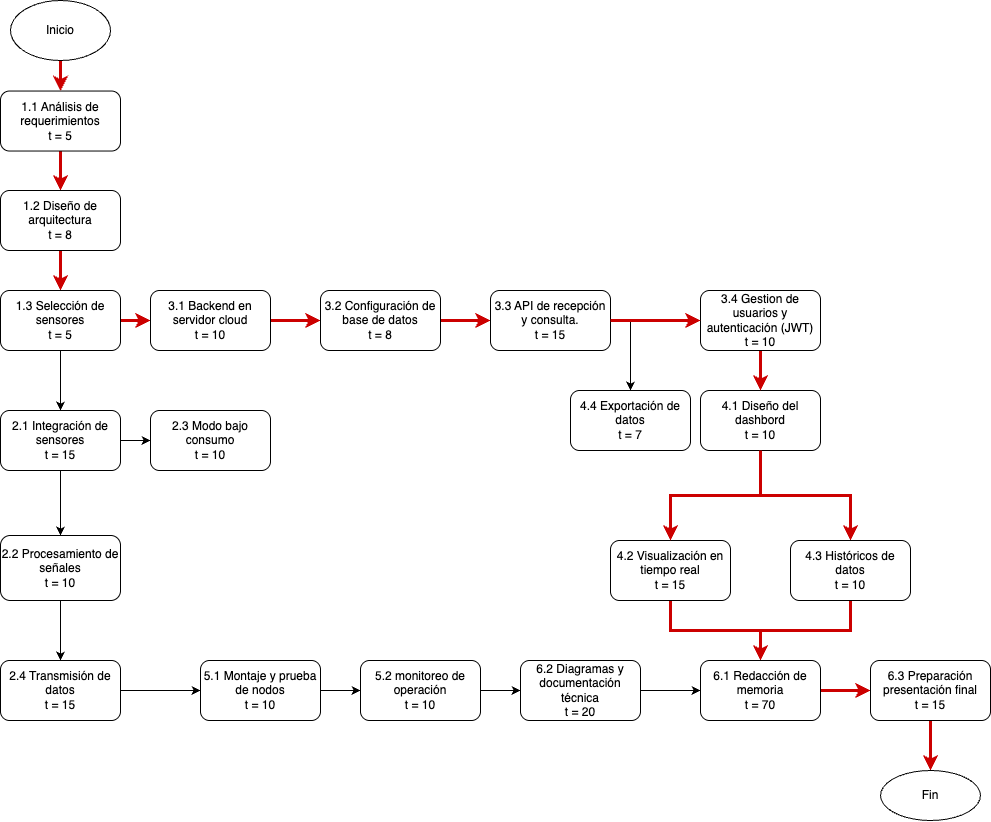
\includegraphics[width=1.05\textwidth]{./Figuras/DiagramAON4.png}
\caption{Diagrama de \textit{Activity on Node}.}
\label{fig:AoN}
\end{figure}
\begin{itemize}
    \item Las líneas más gruesas de color rojo representan la ruta crítica del proyecto.
    \item Las duraciones de las tareas están expresadas en horas.
\end{itemize}

\section{11. Diagrama de Gantt}
\label{sec:gantt}
En la figura 3 se muestra el diagrama de Gantt a nivel general del proyecto.
\begin{figure}[htpb]
    \centering 
    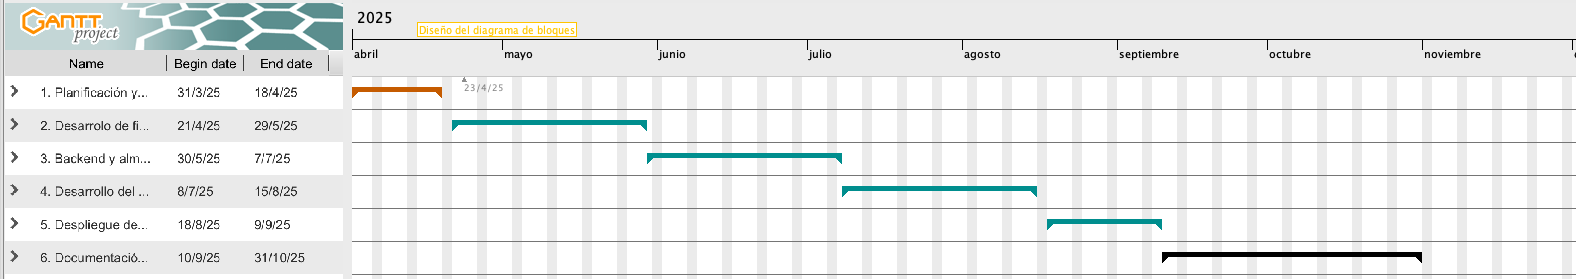
\includegraphics[width=1.05\textwidth]{./Figuras/gantt1.png}
    \caption{Diagrama de Gantt a nivel general del proyecto.}
    \label{fig:AoN}
    \end{figure}

En la figura 4 se muestra el diagrama de Gantt para la planificación y diseño del sistema.
\begin{figure}[htpb]
    \centering 
    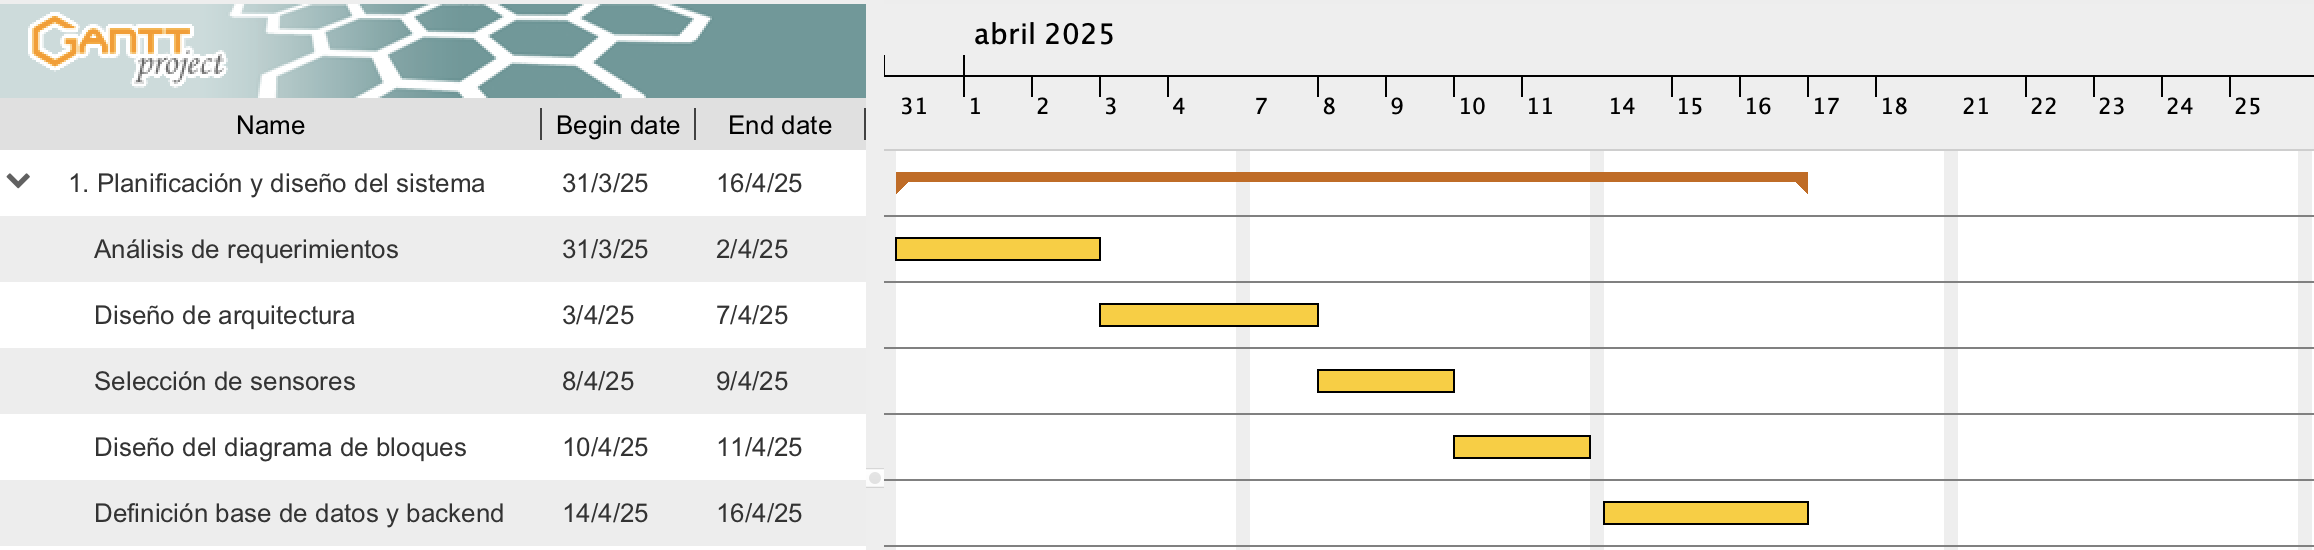
\includegraphics[width=1.05\textwidth]{./Figuras/gantt2.png}
    \caption{Diagrama de Gantt etapa 1.}
    \label{fig:AoN}
    \end{figure}

En la figura 5 se muestra el diagrama de Gantt para el desarrollo del firmware para nodos sensores.
\begin{figure}[htpb]
    \centering 
    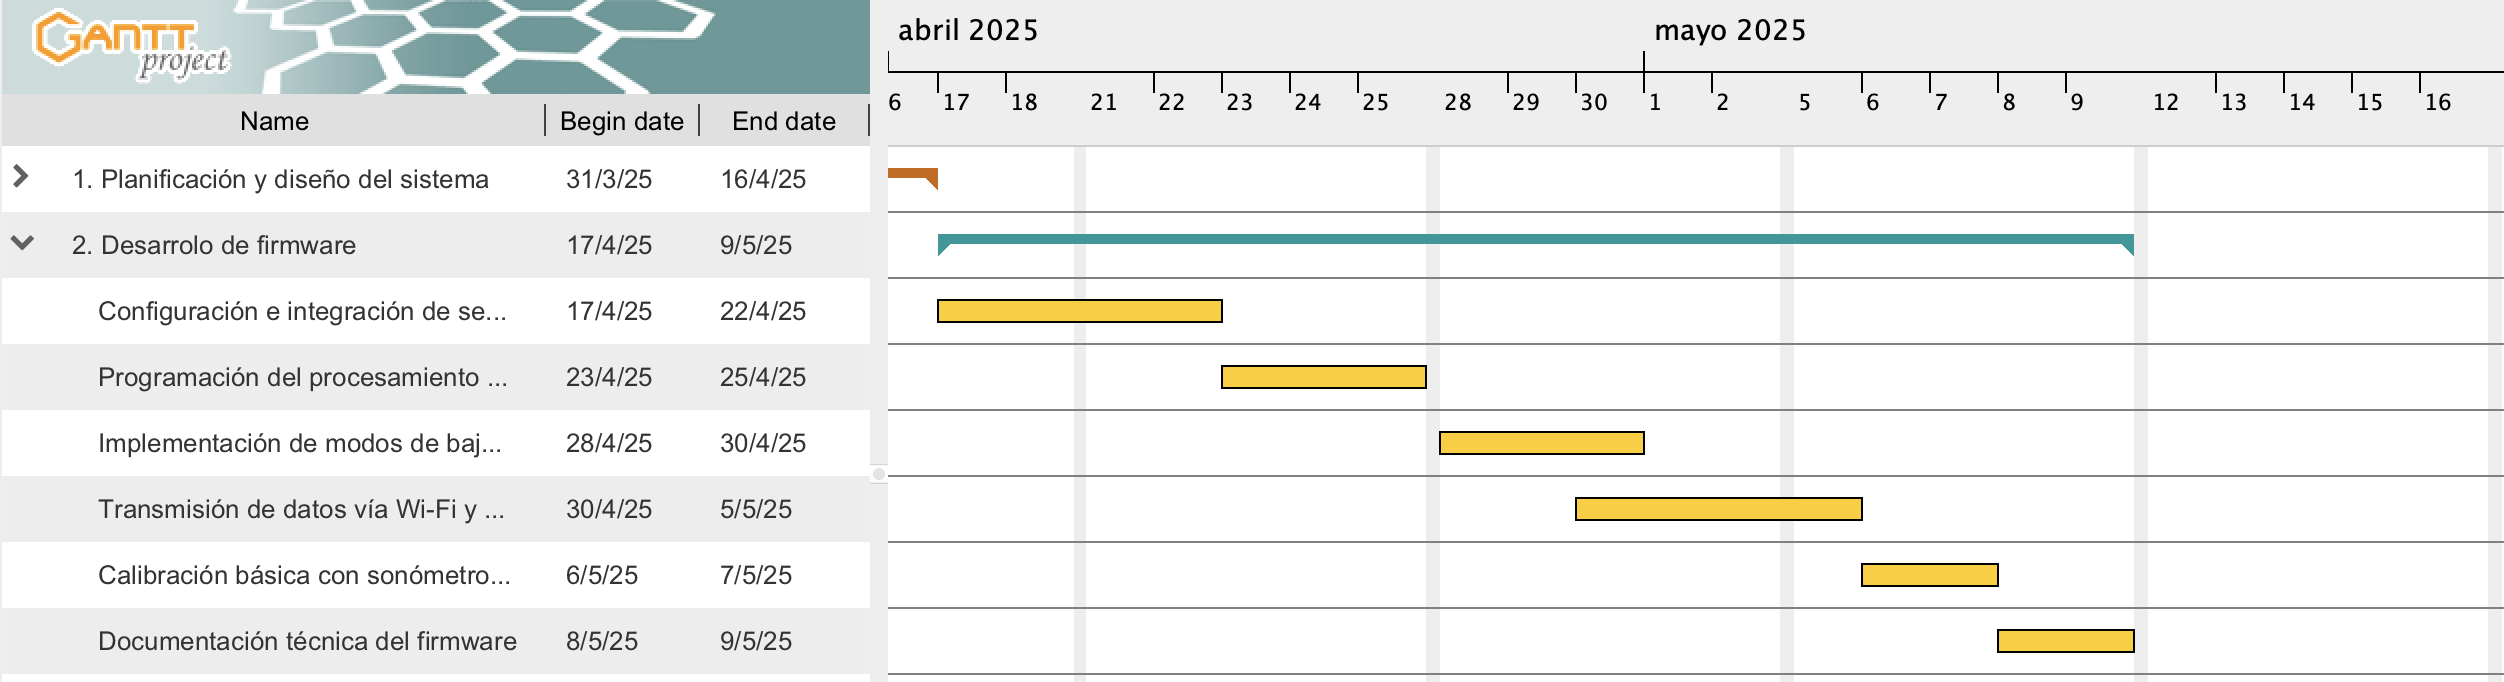
\includegraphics[width=1.05\textwidth]{./Figuras/gantt3.png}
    \caption{Diagrama de Gantt etapa 2.}
    \label{fig:AoN}
    \end{figure}

En la figura 6 se muestra el diagrama de Gantt para el desarrollo de Backend y almacenamiento de datos.
\begin{figure}[htpb]
    \centering 
    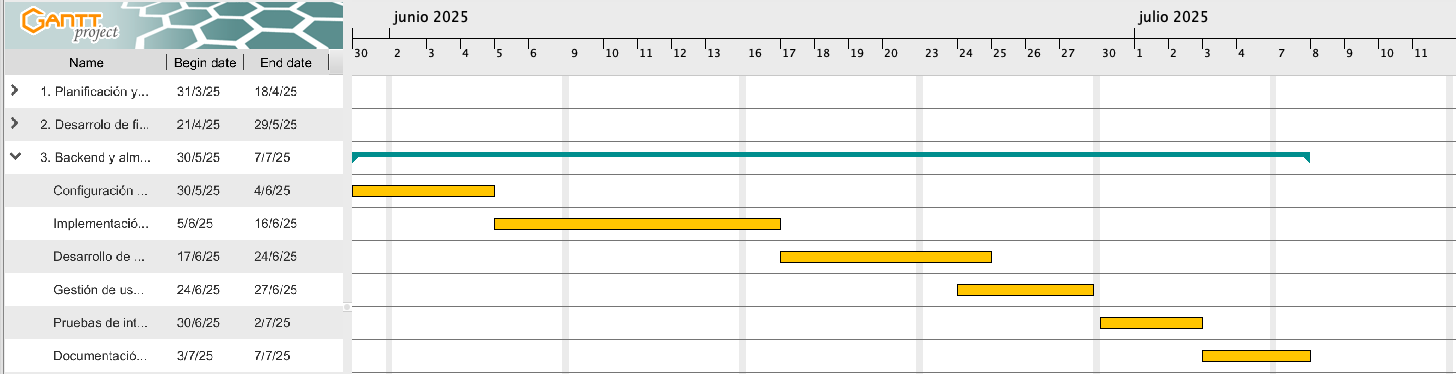
\includegraphics[width=1.05\textwidth]{./Figuras/gantt4.png}
    \caption{Diagrama de Gantt etapa 3.}
    \label{fig:AoN}
    \end{figure}

En la figura 7 se muestra el diagrama de Gantt para el desarrollo del Desarrollo del dashboard web.
\begin{figure}[htpb]
    \centering 
    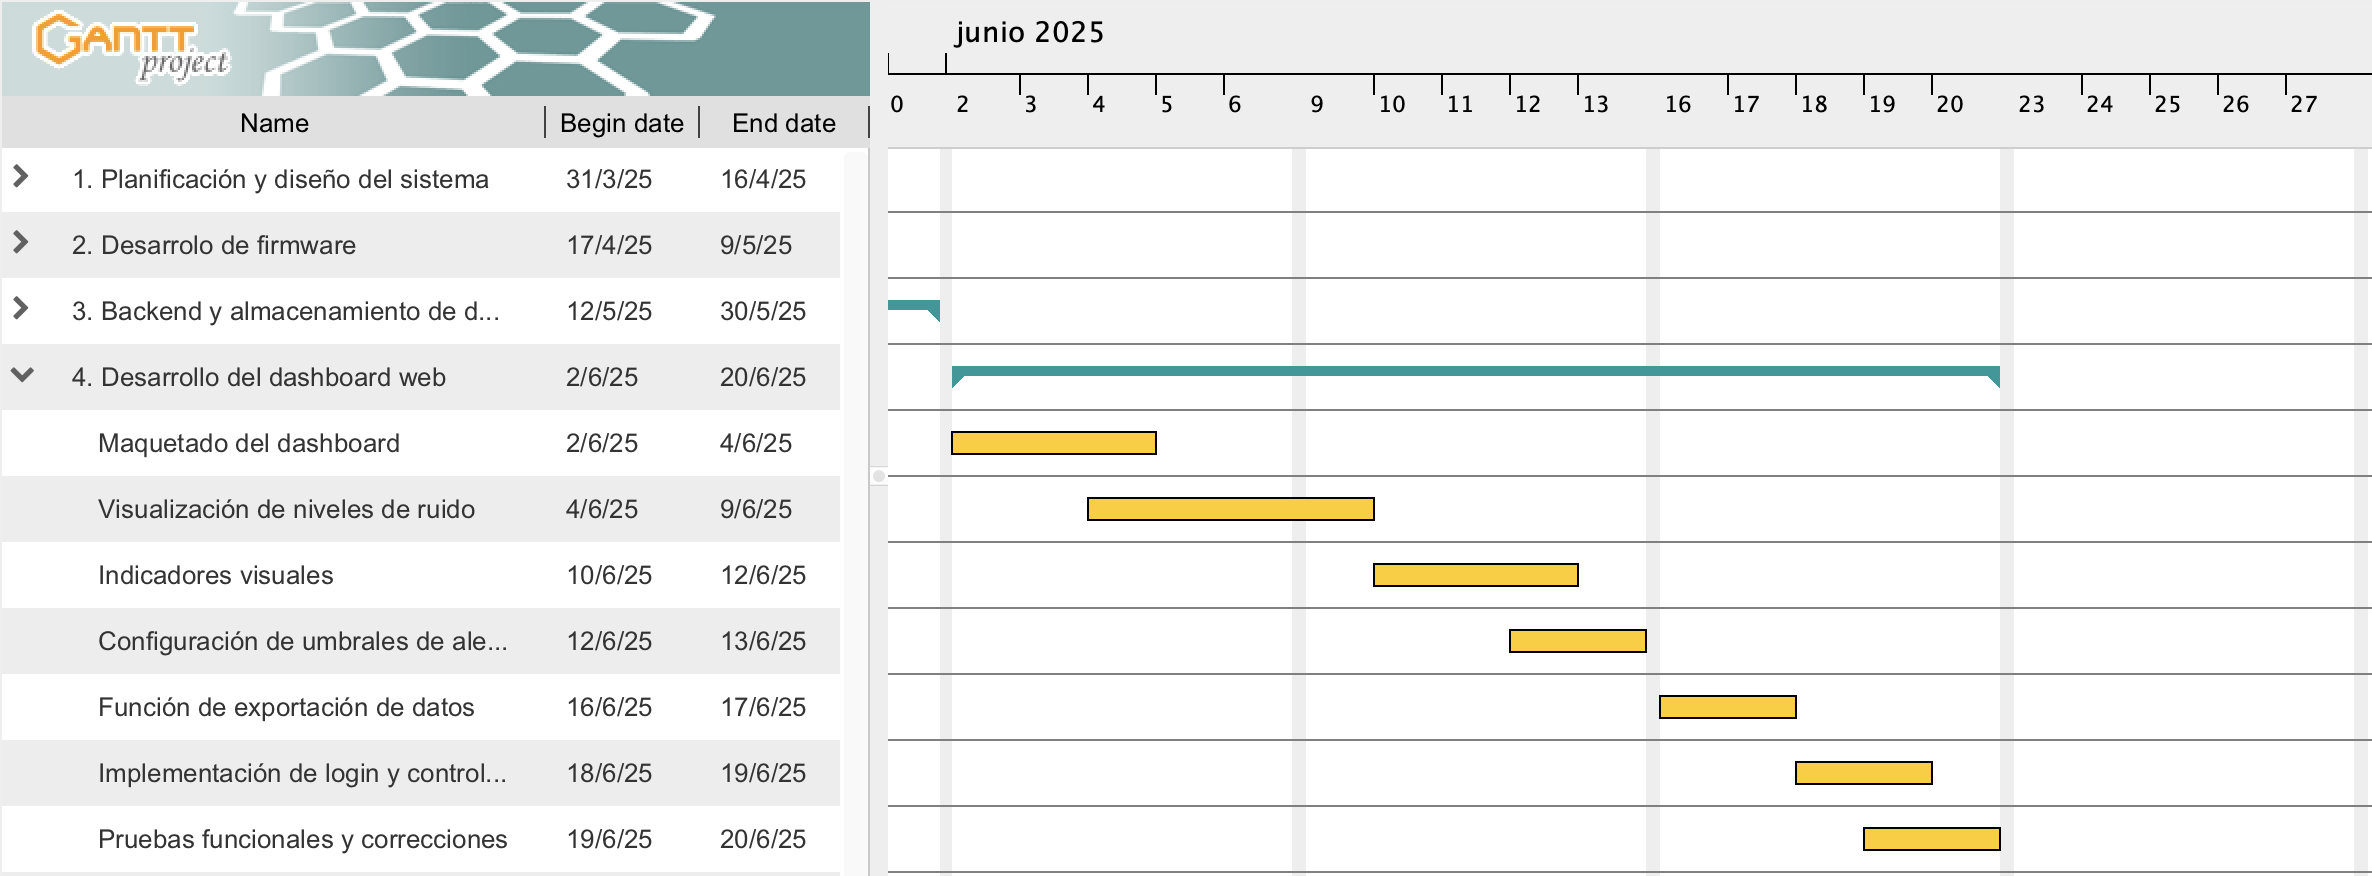
\includegraphics[width=1.05\textwidth]{./Figuras/gantt5.png}
    \caption{Diagrama de Gantt etapa 4.}
    \label{fig:AoN}
    \end{figure}

En la figura 8 se muestra el diagrama de Gantt para el despliegue del prototipo y validación.
\begin{figure}[htpb]
    \centering 
    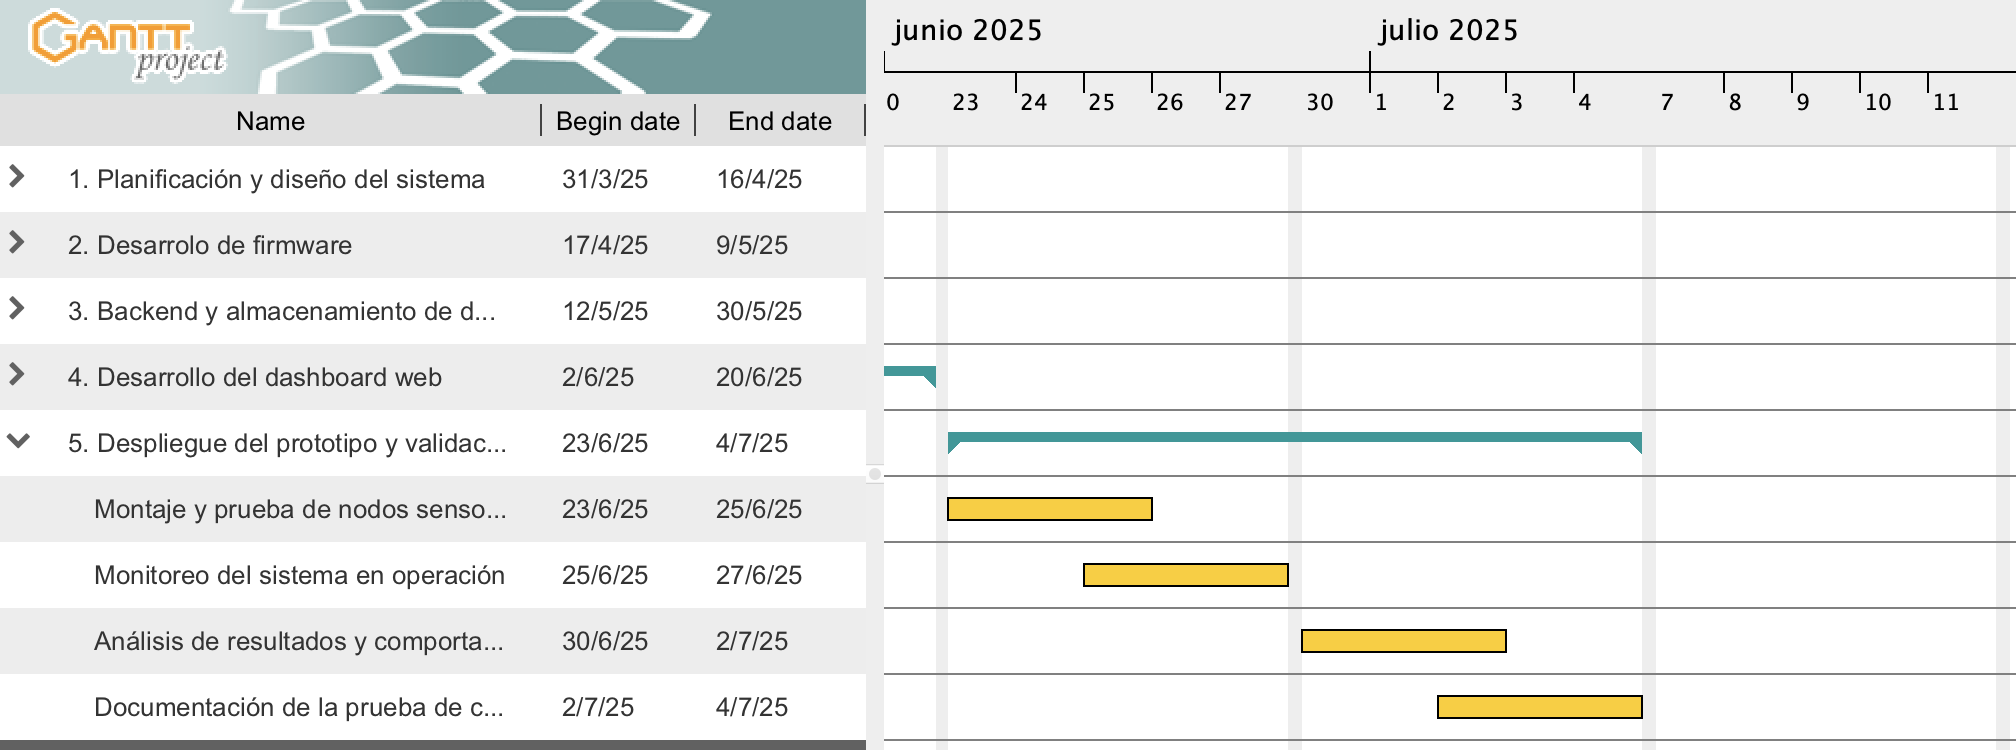
\includegraphics[width=1.05\textwidth]{./Figuras/gantt6.png}
    \caption{Diagrama de Gantt etapa 5.}
    \label{fig:AoN}
    \end{figure}

En la figura 9 se muestra el diagrama de Gantt para el desarrollo de la documentación y entregables.
\begin{figure}[htpb]
    \centering 
    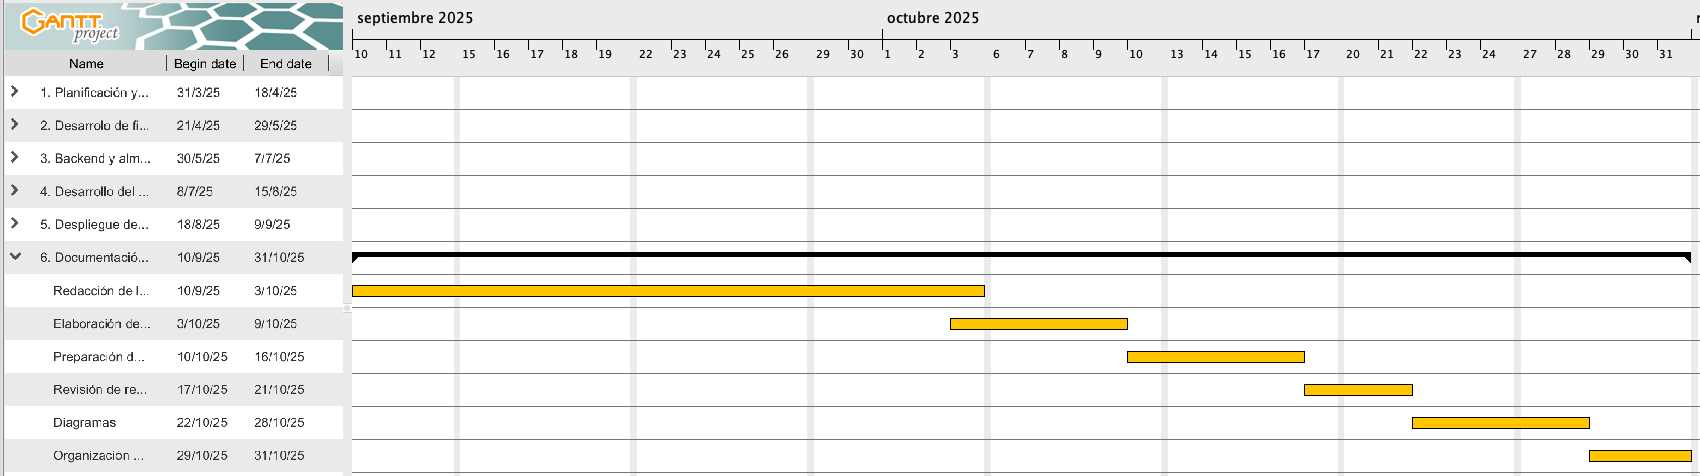
\includegraphics[width=1.05\textwidth]{./Figuras/gantt7.png}
    \caption{Diagrama de Gantt etapa 6.}
    \label{fig:AoN}
    \end{figure}


\section{12. Presupuesto detallado del proyecto}
\label{sec:presupuesto}
Los valores están expresados en pesos argentinos (ARS), cotización abril 2025.

\begin{table}[htpb]
\centering
\begin{tabularx}{\linewidth}{@{}|X|c|r|r|@{}}
\hline
\rowcolor[HTML]{C0C0C0} 
\multicolumn{4}{|c|}{\cellcolor[HTML]{C0C0C0}COSTOS DIRECTOS} \\ \hline
\rowcolor[HTML]{C0C0C0} 
Descripción &
  \multicolumn{1}{c|}{\cellcolor[HTML]{C0C0C0}Cantidad} &
  \multicolumn{1}{c|}{\cellcolor[HTML]{C0C0C0}Valor unitario} &
  \multicolumn{1}{c|}{\cellcolor[HTML]{C0C0C0}Valor total} \\ \hline
  Sensores de ruido (micrófono electret + módulo amplificador)&
  \multicolumn{1}{c|}{3} &
  \multicolumn{1}{c|}{8000} &
  \multicolumn{1}{c|}{24000} \\ \hline
 ESP32 con LoRa&
  \multicolumn{1}{c|}{3} &
  \multicolumn{1}{c|}{17000} &
  \multicolumn{1}{c|}{51000} \\ \hline
  Caja protectora para cada nodo&
  \multicolumn{1}{c|}{3} &
  \multicolumn{1}{c|}{10000} &
  \multicolumn{1}{c|}{30000} \\ \hline
  Base de datos PostgreSQL (uso limitado - estimado equivalente)&
  \multicolumn{1}{c|}{1} &
  \multicolumn{1}{c|}{2000} &
  \multicolumn{1}{c|}{2000} \\ \hline
  Sensor de temperatura/humedad para compensación acústica (DHT22)&
  \multicolumn{1}{c|}{1} &
  \multicolumn{1}{c|}{12000} &
  \multicolumn{1}{c|}{12000} \\ \hline
  Gateway LoRa (alternativa: WisGate Edge Lite 2)&
  \multicolumn{1}{c|}{1} &
  \multicolumn{1}{c|}{85000} &
  \multicolumn{1}{c|}{85000} \\ \hline
  Componentes electrónicos varios (resistencias, jumpers, protoboards)&
  \multicolumn{1}{c|}{1} &
  \multicolumn{1}{c|}{10000} &
  \multicolumn{1}{c|}{10000} \\ \hline

\multicolumn{3}{|c|}{SUBTOTAL} &
  \multicolumn{1}{c|}{214000 ARS} \\ \hline
\rowcolor[HTML]{C0C0C0} 
\multicolumn{4}{|c|}{\cellcolor[HTML]{C0C0C0}COSTOS INDIRECTOS} \\ \hline
\rowcolor[HTML]{C0C0C0} 
Descripción &
  \multicolumn{1}{c|}{\cellcolor[HTML]{C0C0C0}Cantidad} &
  \multicolumn{1}{c|}{\cellcolor[HTML]{C0C0C0}Valor unitario} &
  \multicolumn{1}{c|}{\cellcolor[HTML]{C0C0C0}Valor total} \\ \hline
  Impresión de memoria y presentación&
  \multicolumn{1}{c|}{1} &
  \multicolumn{1}{c|}{15000} &
  \multicolumn{1}{c|}{15000} \\ \hline
  Transporte / imprevistos&
  \multicolumn{1}{c|}{1} &
  \multicolumn{1}{c|}{4000} &
  \multicolumn{1}{c|}{4000} \\ \hline
  30 \% sobre los costos directos&
  \multicolumn{1}{c|}{1} &
  \multicolumn{1}{c|}{64200} &
  \multicolumn{1}{c|}{64200} \\ \hline
\multicolumn{3}{|c|}{SUBTOTAL} &
  \multicolumn{1}{c|}{83200 ARS} \\ \hline
\rowcolor[HTML]{C0C0C0}
\multicolumn{3}{|c|}{TOTAL} &297200 ARS
   \\ \hline
\end{tabularx}%
\caption*{Tabla 1. Presupuesto del proyecto.}
\end{table}


\section{13. Gestión de riesgos}
\label{sec:riesgos}

\begin{consigna}{red}
a) Identificación de los riesgos (al menos cinco) y estimación de sus consecuencias:
 
Riesgo 1: detallar el riesgo (riesgo es algo que si ocurre altera los planes previstos de forma negativa)
\begin{itemize}
	\item Severidad (S): mientras más severo, más alto es el número (usar números del 1 al 10).\\
	Justificar el motivo por el cual se asigna determinado número de severidad (S).
	\item Probabilidad de ocurrencia (O): mientras más probable, más alto es el número (usar del 1 al 10).\\
	Justificar el motivo por el cual se asigna determinado número de (O). 
\end{itemize}   

Riesgo 2:
\begin{itemize}
	\item Severidad (S): X.\\
	Justificación...
	\item Ocurrencia (O): Y.\\
	Justificación...
\end{itemize}

Riesgo 3:
\begin{itemize}
	\item Severidad (S):  X.\\
	Justificación...
	\item Ocurrencia (O): Y.\\
	Justificación...
\end{itemize}


b) Tabla de gestión de riesgos:      (El RPN se calcula como RPN=SxO)

\begin{table}[htpb]
\centering
\begin{tabularx}{\linewidth}{@{}|X|c|c|c|c|c|c|@{}}
\hline
\rowcolor[HTML]{C0C0C0} 
Riesgo & S & O & RPN & S* & O* & RPN* \\ \hline
       &   &   &     &    &    &      \\ \hline
       &   &   &     &    &    &      \\ \hline
       &   &   &     &    &    &      \\ \hline
       &   &   &     &    &    &      \\ \hline
       &   &   &     &    &    &      \\ \hline
\end{tabularx}%
\end{table}

Criterio adoptado: 

Se tomarán medidas de mitigación en los riesgos cuyos números de RPN sean mayores a...

Nota: los valores marcados con (*) en la tabla corresponden luego de haber aplicado la mitigación.

c) Plan de mitigación de los riesgos que originalmente excedían el RPN máximo establecido:
 
Riesgo 1: plan de mitigación (si por el RPN fuera necesario elaborar un plan de mitigación).
  Nueva asignación de S y O, con su respectiva justificación:
  \begin{itemize}
	\item Severidad (S*): mientras más severo, más alto es el número (usar números del 1 al 10).
          Justificar el motivo por el cual se asigna determinado número de severidad (S).
	\item Probabilidad de ocurrencia (O*): mientras más probable, más alto es el número (usar del 1 al 10).
          Justificar el motivo por el cual se asigna determinado número de (O).
	\end{itemize}

Riesgo 2: plan de mitigación (si por el RPN fuera necesario elaborar un plan de mitigación).
 
Riesgo 3: plan de mitigación (si por el RPN fuera necesario elaborar un plan de mitigación).

\end{consigna}


\section{14. Gestión de la calidad}
\label{sec:calidad}

\begin{consigna}{red}
Elija al menos diez requerimientos que a su criterio sean los más importantes/críticos/que aportan más valor y para cada uno de ellos indique las acciones de verificación y validación que permitan asegurar su cumplimiento.

\begin{itemize} 
\item Req \#1: copiar acá el requerimiento con su correspondiente número.

\begin{itemize}
	\item Verificación para confirmar si se cumplió con lo requerido antes de mostrar el sistema al cliente. Detallar.
	\item Validación con el cliente para confirmar que está de acuerdo en que se cumplió con lo requerido. Detallar. 
\end{itemize}

\end{itemize}

Tener en cuenta que en este contexto se pueden mencionar simulaciones, cálculos, revisión de hojas de datos, consulta con expertos, mediciones, etc.  

Las acciones de verificación suelen considerar al entregable como ``caja blanca'', es decir se conoce en profundidad su funcionamiento interno.  

En cambio, las acciones de validación suelen considerar al entregable como ``caja negra'', es decir, que no se conocen los detalles de su funcionamiento interno.

\end{consigna}

\section{15. Procesos de cierre}    
\label{sec:cierre}

\begin{consigna}{red}
Establecer las pautas de trabajo para realizar una reunión final de evaluación del proyecto, tal que contemple las siguientes actividades:

\begin{itemize}
	\item Pautas de trabajo que se seguirán para analizar si se respetó el Plan de Proyecto original:\\
	 - Indicar quién se ocupará de hacer esto y cuál será el procedimiento a aplicar. 
	\item Identificación de las técnicas y procedimientos útiles e inútiles que se emplearon, los problemas que surgieron y cómo se solucionaron:\\
	 - Indicar quién se ocupará de hacer esto y cuál será el procedimiento para dejar registro.
	\item Indicar quién organizará el acto de agradecimiento a todos los interesados, y en especial al equipo de trabajo y colaboradores:\\
	  - Indicar esto y quién financiará los gastos correspondientes.
\end{itemize}

\end{consigna}

\end{document}